\centering
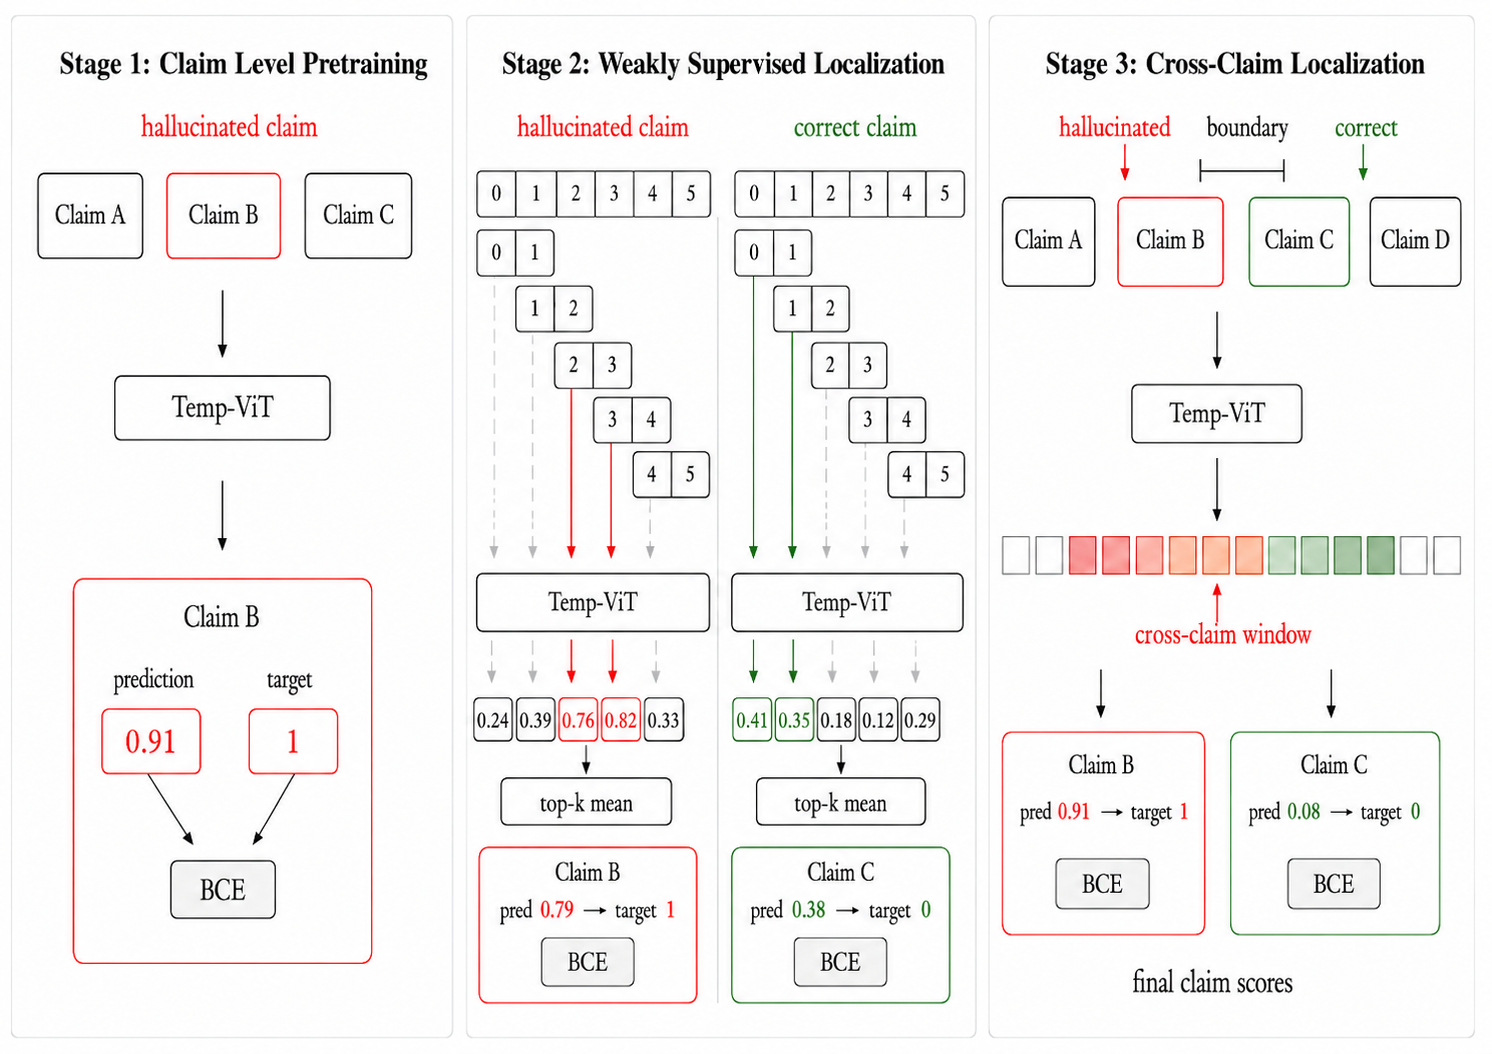
\includegraphics[width=0.95\textwidth]{figs/fig1_overview.png}\par
\captionof{figure}{\textbf{Three-stage Temp-ViT training framework.}
Stage 1 pretrains Temp-ViT to predict an uncertainty label for an
isolated claim span, mapping a labeled claim to a claim-level
prediction with BCE supervision. Stage 2 introduces weakly supervised
localization within individual claims: overlapping token windows are
scored by Temp-ViT, the highest-scoring windows are aggregated with
a top-$k$ mean, and only these selected windows contribute to the
claim-level loss signal. Stage 3 refines the model on full passages containing
adjacent hallucinated and correct claims, exposing Temp-ViT to cross-claim
boundary windows and producing final per-claim uncertainty scores.
Red denotes hallucinated claims or high-uncertainty windows, while
green denotes correct claims or low-uncertainty windows.}
\label{fig:overview}
\vspace{1em}
